\begin{frame}
  \frametitle{Born–von Karman boundary condition}
  \begin{center}
    \resizebox{!}{0.4\textheight}{
    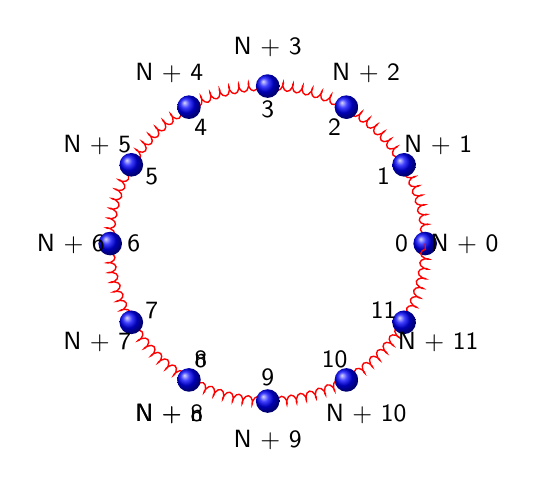
\begin{tikzpicture}
      [
      spring/.style={
        line width=0.5pt,
        decorate,
        decoration={
            coil,
            amplitude=1.5,
            segment length=3.5,
          }
        },
      ]
      \foreach \i in {0,..., 11}{
        \draw[spring, draw=red] (\i*30:2) arc [
          radius=2, start angle=\i * 30, end angle=\i * 30 + 30
        ];
        \shade[ball color=blue] (\i*30:2) circle (0.15);
        \ifthenelse{\i < 5}{
          \node[] at (\i * 30 : 1.7) {\small\textsf{\i}};
          \node[] at (\i * 30 : 2.5) {\small\textsf{N + \i}};
        }{}
      }
      \node[] at (8 * 30 : 1.7) {\small\textsf{n}};
      \node[] at (8 * 30 : 2.5) {\small\textsf{N + n}};
    \end{tikzpicture}
    }
  \end{center}

  The Born-von Karman Periodic Boundary Condition:
  \begin{equation*}
    u_{n} = u_{N+n}
    \quad
    \Rightarrow
    \quad
    e^{iqx_j} = e^{iqx_{N+j}} 
    \quad
    \Rightarrow
    \quad
    e^{iqNa} = 1
    \quad
    \Rightarrow
    \quad
    q = \frac{2 \pi}{a} \frac{l}{N}
  \end{equation*}

\end{frame}

%%% Local Variables:
%%% mode: latex
%%% TeX-master: t
%%% End:
